\documentclass[10pt]{article}
\usepackage[UTF8]{ctex}

\usepackage[utf8]{inputenc} % allow utf-8 input
\usepackage{amsthm}
\usepackage{amsmath,amscd}
\usepackage{amssymb,array}
\usepackage{amsfonts,latexsym}
\usepackage{graphicx,subfig,wrapfig}
\usepackage{times}
\usepackage{psfrag,epsfig}
\usepackage{verbatim}
\usepackage{tabularx}
\usepackage[pagebackref=true,breaklinks=true,letterpaper=true,colorlinks,bookmarks=false]{hyperref}
\usepackage{cite}
\usepackage{algorithm}
\usepackage{multirow}
\usepackage{caption}
\usepackage{diagbox}

\captionsetup[figure]{labelformat=default,labelsep=period,name=Figure}

\usepackage{algorithmic}
%\usepackage[amsmath,thmmarks]{ntheorem}
\usepackage{listings}
\usepackage{color}
\usepackage{bm}

% support llbracket and rrbracket  []
\usepackage{stmaryrd}


\newtheorem{thm}{Theorem}
\newtheorem{mydef}{Definition}

\DeclareMathOperator*{\rank}{rank}
\DeclareMathOperator*{\trace}{trace}
\DeclareMathOperator*{\acos}{acos}
\DeclareMathOperator*{\argmax}{argmax}


\renewcommand{\algorithmicrequire}{ \textbf{Input:}}
\renewcommand{\algorithmicensure}{ \textbf{Output:}}
\renewcommand{\mathbf}{\boldsymbol}
\newcommand{\mb}{\mathbf}
\newcommand{\matlab}[1]{\texttt{#1}}
\newcommand{\setname}[1]{\textsl{#1}}
\newcommand{\Ce}{\mathbb{C}}
\newcommand{\Ee}{\mathbb{E}}
\newcommand{\Ne}{\mathbb{N}}
\newcommand{\Se}{\mathbb{S}}
\newcommand{\norm}[2]{\left\| #1 \right\|_{#2}}

\newenvironment{mfunction}[1]{
	\noindent
	\tabularx{\linewidth}{>{\ttfamily}rX}
	\hline
	\multicolumn{2}{l}{\textbf{Function \matlab{#1}}}\\
	\hline
}{\\\endtabularx}

\newcommand{\parameters}{\multicolumn{2}{l}{\textbf{Parameters}}\\}

\newcommand{\fdescription}[1]{\multicolumn{2}{p{0.96\linewidth}}{

		\textbf{Description}

		#1}\\\hline}

\newcommand{\retvalues}{\multicolumn{2}{l}{\textbf{Returned values}}\\}
\def\0{\boldsymbol{0}}
\def\b{\boldsymbol{b}}
\def\bmu{\boldsymbol{\mu}}
\def\e{\boldsymbol{e}}
\def\u{\boldsymbol{u}}
\def\x{\boldsymbol{x}}
\def\v{\boldsymbol{v}}
\def\w{\boldsymbol{w}}
\def\N{\boldsymbol{N}}
\def\X{\boldsymbol{X}}
\def\Y{\boldsymbol{Y}}
\def\A{\boldsymbol{A}}
\def\B{\boldsymbol{B}}
\def\y{\boldsymbol{y}}
\def\cX{\mathcal{X}}
\def\Var{\mathrm{Var}}
\def\transpose{\top} % Vector and Matrix Transpose

%\long\def\answer#1{{\bf ANSWER:} #1}
\long\def\answer#1{}
\newcommand{\myhat}{\widehat}
\long\def\comment#1{}
\newcommand{\eg}{{e.g.,~}}
\newcommand{\ea}{{et al.~}}
\newcommand{\ie}{{i.e.,~}}

\newcommand{\db}{{\boldsymbol{d}}}
\renewcommand{\Re}{{\mathbb{R}}}
\newcommand{\Pe}{{\mathbb{P}}}

\hyphenation{MATLAB}

\usepackage[margin=1in]{geometry}

\newcounter{ProblemCounter}
\newcounter{oldvalue}
\newcommand{\problem}[2][-1]{
	\setcounter{oldvalue}{\value{secnumdepth}}
	\setcounter{secnumdepth}{0}
	\ifnum#1>0
		\setcounter{ProblemCounter}{#1}
	\else
		\stepcounter{ProblemCounter}
	\fi
	\section{Problem \arabic{ProblemCounter}: #2}
	\setcounter{secnumdepth}{\value{oldvalue}}
}
\newcommand{\subproblem}[1]{
	\setcounter{oldvalue}{\value{section}}
	\setcounter{section}{\value{ProblemCounter}}
	\subsection{#1}
	\setcounter{section}{\value{oldvalue}}
}



\begin{document}

\title{	Fundamentals of Information Theory \\Homework 3}
\date{Due 23:59 (CST), Nov. 2, 2024 }

\author{
    Name: \textbf{Zhou Shouchen} \\
	Student ID: 2021533042
}

\maketitle

\newpage
%===============================
\textcolor{blue}{Problem 1}

2.16 Bottleneck. Suppose that a (nonstationary) Markov chain starts in one of $n$ states, necks down to $k<n$ states, and then fans back to $m>k$ states. Thus, $X_1 \rightarrow X_2 \rightarrow X_3$, that is $p\left(x_1, x_2, x_3\right)=p\left(x_1\right) p\left(x_2 \mid x_1\right) p\left(x_3 \mid x_2\right)$, for all $x_1 \in\{1,2, \ldots, n\}, x_2 \in\{1,2, \ldots, k\}, x_3 \in\{1,2, \ldots, m\}$.

(a) Show that the dependence of $X_1$ and $X_3$ is limited by the bottleneck by proving that $I\left(X_1 ; X_3\right) \leq \log k$.

(b) Evaluate $I\left(X_1 ; X_3\right)$ for $k=1$, and conclude that no dependence can survive such a bottleneck.

\textcolor{blue}{Solution}

(a) Since $X_1 \rightarrow X_2 \rightarrow X_3$ form the Markov chain, so we can get that:
\begin{align*}
I(X_1;X_3) &\leq I(X_1;X_2) \text{\ \ \ (Data Processing Inequality)} \\
&\leq H(X_2) \text{\ \ \ \ \ \ \ (property of mutual information)} \\
&\leq \log k \text{\ \ \ \ \ \ \ \ \ \ ($|X_2|=k$)} \qed
\end{align*}

(b) Since $k=1$, from (a), we can get that
$$I(X_1;X_3) \leq \log 1 = 0$$
And from the property of mutual information, we can get that
$$I(X_1;X_3) \geq 0$$
So we can conclude that $I(X_1;X_3) = 0$.\\
Which means that no dependence can survive such a bottleneck.

\newpage
\textcolor{blue}{Problem 2}

2.3 Minimum entropy. What is the minimum value of $H\left(p_1, \ldots, p_n\right)=H(\mathbf{p})$ as $\mathbf{p}$ ranges over the set of $n$-dimensional probability vectors? Find all $\mathbf{p}$ 's that achieve this minimum.

\textcolor{blue}{Solution}



\newpage
\textcolor{blue}{Problem 3}

8.8 Channel with uniformly distributed noise. Consider a additive channel whose input alphabet $\mathcal{X}=\{0, \pm 1, \pm 2\}$ and whose output $Y=X+Z$, where $Z$ is distributed uniformly over the interval $[-1,1]$. Thus, the input of the channel is a discrete random variable, whereas the output is continuous. Calculate the capacity $C=$ $\max\limits_{p(x)} I(X ; Y)$ of this channel.

\textcolor{blue}{Solution}

Since $Z\sim\text{Unif}[-1,1]$, we have $f_Z(z)=\dfrac{1}{2},z\in[-1,1]$. So we have:
$$h(Z)=\int_{-1}^{1}f_Z(z)\log\dfrac{1}{f_Z(z)}dz=\log\left(1-(-1)\right)=\log 2=1\text{ bit}$$
So we can get that:
\begin{align*}
I(X;Y) &= h(Y)-h(Y|X) \\
&= h(Y) - h(Z|X) \qquad \text{(since $Y=X+Z$)} \\
&= h(Y) - h(Z) \qquad\quad\ \text{(since $Z$ is independent of $X$)} \\
&= h(Y) - 1
\end{align*}
Let $p_i=p(X=i)$, then we can get that:
$$f_Y(y) = \sum_{x\in\mathcal{X}}f_Z(y-x)p(X=x)=\begin{cases}
\frac{1}{2}p_{-2}, & -3\leq y\leq -2 \\
\frac{1}{2}p_{-2}+\frac{1}{2}p_{-1}, & -2<y\leq -1 \\
\frac{1}{2}p_{-1}+\frac{1}{2}p_0, & -1<y\leq 0 \\
\frac{1}{2}p_0+\frac{1}{2}p_1, & 0<y\leq 1 \\
\frac{1}{2}p_1+\frac{1}{2}p_2, & 1<y\leq 2 \\
\frac{1}{2}p_2, & 2<y\leq 3
\end{cases}$$

As we have proved in \textcolor{blue}{Problem 2}: if $Y$ is a continous variable in range $[a,b]$, then $h(Y)_{\max}=\log (b-a)$. If and only if $Y\sim\text{Unif}(a,b)$. \\
So to reach the $h(Y)_{\max}$, we need to make $f_Y(y)=\dfrac{1}{6}$, $y\in[-3,3]$. \\
So we have
$$p_{-2}=p_2=\dfrac{1}{3}, p_{-1}=p_1=0, p_0=\dfrac{1}{3}$$

So above all, we have proved that when $p(x)=\left(\dfrac{1}{3},0,\dfrac{1}{3},0,\dfrac{1}{3}\right)$
$$C=\max_{p(x)}I(X;Y)=h(Y)-1=\log 3\text{ bits}$$

\newpage
\textcolor{blue}{Problem 4}

9.6 Parallel channels and water-filling. Consider a pair of parallel Gaussian channels:
$$\left(\begin{array}{c}Y_1 \\ Y_2 \end{array}\right)=\left(\begin{array}{c}X_1 \\ X_2 \end{array}\right)+\left(\begin{array}{c}Z_1 \\ Z_2 \end{array}\right)$$

where

$$\left(\begin{array}{c}Z_1 \\ Z_2 \end{array}\right) \sim \mathcal{N}\left(0,\left[\begin{array}{cc}
\sigma_1^2 & 0 \\
0 & \sigma_2^2
\end{array}\right]\right)$$

and there is a power constraint $\mathbb{E}\left(X_1^2+X_2^2\right) \leq 2 P$. Assume that $\sigma_1^2>\sigma_2^2$. At what power does the channel stop behaving like a single channel with noise variance $\sigma_2^2$, and begin behaving like a pair of channels?

\textcolor{blue}{Solution}

From what we have learned about the parallel channels, we know that the capacity of the parallel channels is
$$C=\sum_{i=1}^2\dfrac{1}{2}\log\left(1+\dfrac{P_i}{\sigma_i^2}\right)$$
Where $\sum\limits_{i=1}^2P_i\leq 2P$. \\
And with water-filling method, we have $P_i=\left(\nu-\sigma_i^2\right)_+$, $P_1+P_2\leq 2P$ and $\nu$ is the water level, $(\cdot)_+=\max(\cdot, 0)$.

Since $\sigma_1^2>\sigma_2^2$, so

1. When $\nu\in(\sigma_2^2,\sigma_1^2]\Rightarrow P_1=0,P_2=\nu-\sigma_2^2$ \\
$\Rightarrow 2P=P_1+P_2\in(0,\sigma_1^2-\sigma_2^2)$ \\
So when $0\leq P\leq \dfrac{\sigma_1^2-\sigma_2^2}{2}$, the channel behaves like a single channel with noise variance $\sigma_2^2$.

2. When $\nu>\sigma_1^2$, we have $P_1=\nu-\sigma_1^2>0,P_2=\nu-\sigma_2^2>0$ \\
$\Rightarrow 2P=P_1+P_2>2\nu-\sigma_1^2-\sigma_2^2>\sigma_1^2-\sigma_2^2$ \\
So when $P>\dfrac{\sigma_1^2-\sigma_2^2}{2}$, the channel behaves like a pair of channels.

So when $P=\dfrac{\sigma_1^2-\sigma_2^2}{2}$, the channel stops behaving like a single channel with noise variance $\sigma_2^2$, and begins behaving like a pair of channels.

\newpage
\textcolor{blue}{Problem 5}

7.34 Capacity. Find the capacity of \\
(a) Two parallel BSCs: \\
(b) BSC and a single symbol: \\
(c) BSC and a ternary channel:
\begin{figure}[htbp]
    \centering
	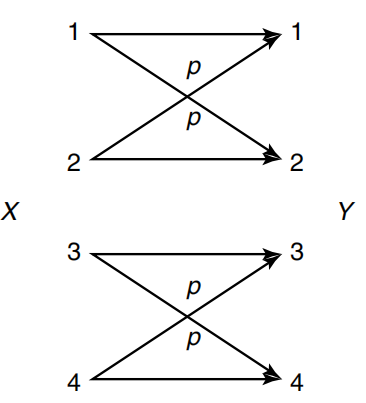
\includegraphics[width=0.3\textwidth]{../figures/7.34_a.png}
	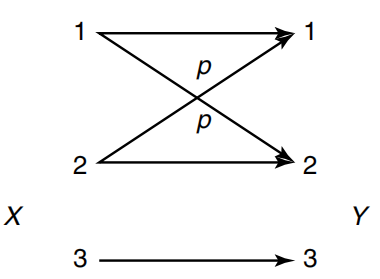
\includegraphics[width=0.3\textwidth]{../figures/7.34_b.png}
	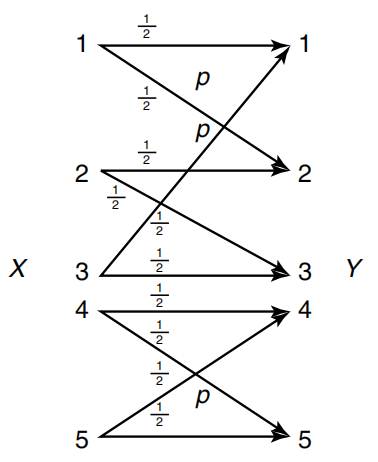
\includegraphics[width=0.3\textwidth]{../figures/7.34_c.png}
\end{figure}

(d) Ternary channel:
$$
p(y|x)=\left(\begin{array}{lll}
\frac{2}{3} & \frac{1}{3} & 0 \\
0 & \frac{1}{3} & \frac{2}{3}
\end{array}\right)
$$

\textcolor{blue}{Solution}

Since for (a), (b), (c): the channels are all combined with two parallel channels, so we can introduce two Lemmas.


Lemma1: If the channel is combined with two parallel channels with probability $\pi$ to the first channel, and $1-\pi$ to the second channel, which is as followed.
\begin{figure}[htbp]
    \centering
	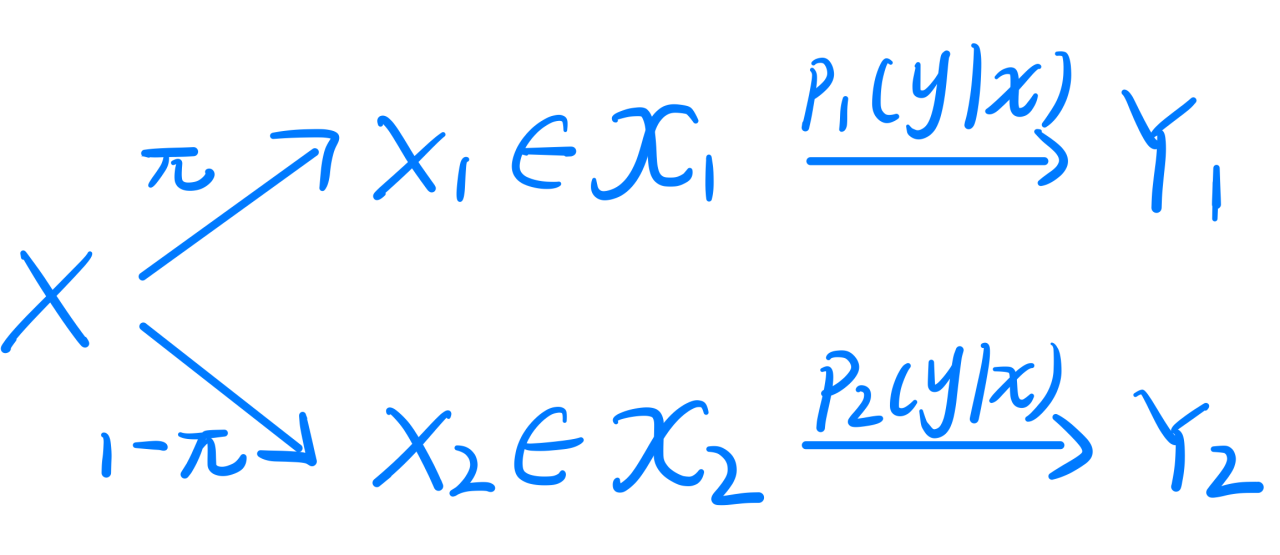
\includegraphics[width=0.3\textwidth]{../figures/parallel.png}
\end{figure}

Suppose the channel capacity of the total channel is $C$, and the capacity of the two channels are $C_1$ and $C_2$ respectively. Then we have
$$2^C=2^{C_1}+2^{C_2}$$
Proof: \\
Let $\Theta(X)$ be the auxiliary variable, indicating that $X$ is send to the $\Theta(X)$'s channel. Then we have
\begin{align*}
\Theta(X) &= \begin{cases}
1 & , X\in \mathcal{X}_1 \\
2 & , X\in \mathcal{X}_2 \\
\end{cases} \\
C_1 &= \max_{p_1(x)}I(X_;Y_1) \\
C_2 &= \max_{p_2(x)}I(X_;Y_2)
\end{align*}
And we also have that $p(\Theta=1)=p(X\in\mathcal{X}_1)=\pi, p(\Theta=2)=p(X\in\mathcal{X}_2)=1-\pi$.
And since when given $Y$ or given $X$, we could know $\Theta$, so we have $I(X;\Theta|Y)=H(\Theta|Y)-H(\Theta|X,Y)=0$.
i.e.
\begin{align*}
I(X;Y,\Theta) &= I(X;\Theta) + I(X;Y|\Theta) \\
&= I(X;Y) + I(X;\Theta|Y) = I(X;Y)
\end{align*}
Then we have
\begin{align*}
I(X;Y) &= I(X;\Theta) + I(X;Y|\Theta) \\
&= H(\Theta) - H(\Theta|X) + I(X;Y|\Theta) \\
&= H(\Theta) + I(X;Y|\Theta) \text{\qquad\qquad\quad ($\Theta$ is deterministic when $X$ is given)} \\
&= H\left(\pi,1-\pi\right) + I(X;Y|\Theta)
\end{align*}
As for $I(X;Y|\Theta)$, we have
\begin{align*}
I(X;Y|\Theta) &= H(X|\Theta) - H(X|Y,\Theta) \\
&= \sum_{\theta}p(\Theta=\theta)H(X|\Theta=\theta) - \sum_{\theta}p(\Theta=\theta)H(X|Y,\Theta=\theta) \\
&= \sum_{\theta}p(\Theta=\theta)\left[H(X|\Theta=\theta) - H(X|Y,\Theta=\theta)\right] \\
&= \sum_{\theta}p(\Theta=\theta)I(X;Y|\Theta=\theta) \\
&= \pi I(X_1;Y_1) + (1-\pi)I(X_2;Y_2) \\
&\leq \pi C_1 + (1-\pi)C_2 \text{\qquad\qquad ($C_1$ and $C_2$ are the capacity of the two channels)}
\end{align*}
So we have
$$I(X;Y) \leq H(\pi,1-\pi) \pi C_1 + (1-\pi)C_2 = -\pi\log \pi - (1-\pi)\log(1-\pi) + \pi C_1 + (1-\pi)C_2 \triangleq f(\pi)$$
Since we want to maximize $f(\pi)$, so it is obviously that $\pi=0$ or $\pi=1$ is not the optimal solution. And from the property of capcity, we have $C_1,C_2\geq 0$, so we have
\begin{align*}
f'(\pi) &= \log(1-\pi)-\log\pi+C_1-C_2 \\
f''(\pi) &= -\log_e2\left(\dfrac{1}{1-\pi}+\dfrac{1}{\pi}\right) < 0
\end{align*}
So $f(\pi)$ is a concave function, so the optimal solution is
$$f'(\pi^*)=0\Rightarrow \pi^*=\dfrac{2^{C_1}}{2^{C_1}+2^{C_2}}$$
So we have
\begin{align*}
C &= \max_{p(x)}I(X;Y) = \max_{\pi} f(\pi) = f(\pi^*) \\
&= \log \left(2^{C_1}+2^C_2\right)
\end{align*}
So we have proved that $2^C=2^{C_1}+2^{C_2}$. \qed

Lemma2: For a BSC. The probability of error is $p$, then the capacity is $1-H(p,1-p)$.
\begin{figure}[htbp]
    \centering
	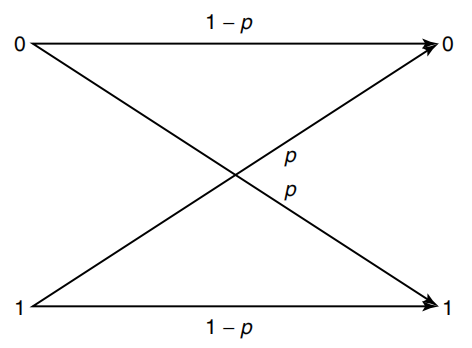
\includegraphics[width=0.3\textwidth]{../figures/BSC.png}
\end{figure}
\begin{align*}
I(X;Y) &= H(Y) - H(Y|X) \\
&= H(Y)-\sum_{x}p(x)H(Y|X=x) \\
&= H(Y) - H(p,1-p) \\
&\leq 1 - H(p,1-p)
\end{align*}
And we have when $P(X=1)=P(X=2)=\dfrac{1}{2}$, then $P(Y=0)=\sum\limits_xP(X=x)P(Y=1|X=x)=\dfrac{1}{2}$, and so does $P(Y=1)$.

So the inequality takes the equality, so we have when $p(x)=\left(\dfrac{1}{2},\dfrac{1}{2}\right)$
$$C=\max_{p(x)}I(X;Y)=1-H(p,1-p)$$
So with the two Lemmas, we could solve the problem easier. \\

(a) The two channels are paralleled BSC, so we have $C_1=C_2=1-H(p,1-p)$, so we have
$$C=\log\left(2^{1-H(p,1-p)}+2^{1-H(p,1-p)}\right)=2-H(p,1-p)$$

Where $\pi^*=\dfrac{2^{C_1}}{2^{C_1}+2^{C_2}}=\dfrac{1}{2}$.

When $p(x)=\left(\dfrac{1}{4},\dfrac{1}{4},\dfrac{1}{4},\dfrac{1}{4}\right)$, $I(X;Y)$ could take the maximum value.

(b) The first channel is a BSC, so $C_1=1-H(p,1-p)$. And for the second channel, $Y_2=X_2=3$, so
$$I(X_2;Y_2)=H(X_2)-H(X_2|Y_2)=H(X_2)=0$$
i.e. $C_2=0$. So we have
$$C=\log\left(2^{1-H(p,1-p)}+2^0\right)=\log\left(2^{1-H(p,1-p)}+1\right)$$

Where $\pi^*=\dfrac{2^{C_1}}{2^{C_1}+2^{C_2}}=\dfrac{2}{2+2^{H\left(p,1-p\right)}}$.

When $p(x)=\left(\dfrac{1}{2+2^{H\left(p,1-p\right)}},\dfrac{1}{2+2^{H\left(p,1-p\right)}},\dfrac{2^{H\left(p,1-p\right)}}{2+2^{H\left(p,1-p\right)}}\right)$, $I(X;Y)$ could take the maximum value. \\\\


(c) The second channel is a BSC, and $p=\dfrac{1}{2}$, so $C_2=1-H(p,1-p)=0$.

And for the first channel:
\begin{align*}
I(X;Y) &= H(Y) - H(Y|X) \\
&= H(Y) - \sum_{x}p(x)H(Y|X=x) \\
&= H(Y) - \sum_{x}p(x)H\left(\dfrac{1}{2},\dfrac{1}{2}\right) \\
&= H(Y) - 1 \\
&\leq \log 3 - 1
\end{align*}
When $p(X=1)=p(X=2)=p(X=3)=\dfrac{1}{3}$, we have
$$P(Y=1)=\sum_xP(X=x)P(Y=1|X=x)=\dfrac{1}{3}$$
Similarly, $P(Y=2)=P(Y=3)=\dfrac{1}{3}$. So the inequality takes the equality, so we have $C_1=\log 3 - 1$. \\
So we have
$$C=\log\left(2^0+2^{\log 3-1}\right)=\log 5 - 1$$

Where $\pi^*=\dfrac{2^{C_1}}{2^{C_1}+2^{C_2}}=\dfrac{3}{5}$ bit per transmission.

When $p(x)=\left(\dfrac{1}{5},\dfrac{1}{5},\dfrac{1}{5},\dfrac{1}{5},\dfrac{1}{5}\right)$, $I(X;Y)$ could take the maximum value.

(d)
\begin{align*}
I(X;Y) &= H(Y) - H(Y|X) \\
&= H(Y) - \sum_{x}p(x)H(Y|X=x) \\
&= H(Y) - H\left(\dfrac{1}{3},\dfrac{2}{3}\right) \\
&\leq \log 3 - H\left(\dfrac{1}{3},\dfrac{2}{3}\right)
\end{align*}
When $p(X=1)=p(X=2)=p(X=3)=\dfrac{1}{3}$, we have
$$P(Y=1)=\sum_xP(X=x)P(Y=1|X=x)=\dfrac{1}{3}$$
Similarly, $P(Y=2)=P(Y=3)=\dfrac{1}{3}$. So the inequality takes the equality. \\
So we have $C=\log 3 - H\left(\dfrac{1}{3},\dfrac{2}{3}\right)$. \\
And we have
$$H\left(\dfrac{1}{3},\dfrac{2}{3}\right) = -\dfrac{1}{3}\log\dfrac{1}{3}-\dfrac{2}{3}\log\dfrac{2}{3} = \log 3 - \dfrac{2}{3}$$

So above all, we have $C=\dfrac{2}{3}$ bit per transmission.

\newpage

\end{document}